\documentclass[11pt,letterpaper,boxed]{hmcpset}
\usepackage{fullpage}
\setlength{\parskip}{6pt}
\setlength{\parindent}{0pt}
\usepackage[margin=1in]{geometry}
\usepackage{graphicx}
\usepackage{enumerate}
\usepackage{marvosym}
\usepackage{amssymb}
\usepackage{wasysym}
\usepackage{gensymb}
\usepackage{mathrsfs}
\usepackage{scrextend}
\usepackage{mathtools}
\usepackage{pgfplots}
\usepackage{xspace}

\name{Name $\rule{4cm}{0.15mm}$}
\class{Physics 51 Section $\rule{.5cm}{0.15mm}$ Box \# $\rule{1cm}{0.15mm}$}
\assignment{Problem Set 5}
\duedate{8 October 2018}

\begin{document}

%\begin{center}
\noindent\textbf{Collaborators:} 
%\end{center} 

%\problemlist{}

\begin{problem}[HRK P29.5 Solo]
$(a)$ The current density across a cylindrical conductor of radius $R$ varies according to the equation
$$ j = j_0(1-r/R)$$
where $r$ is the distance from the axis. Thus the current density is a maximum $j_0$ at the axis $r=0$ and decreases linearly to zero at the surface $r=R$. Calculate the current in terms of $j_0$ and the conductor's cross-sectional area $A= \pi R^2$. $(b)$ Suppose that, instead, the current density is a maximum $j_0$ at the surface and decreases linearly to zero at the axis so that $$ j = j_0r/R$$ Calculate the current. Why is the result different from $(a)$?
\end{problem}

\begin{solution}
\vfill
\end{solution}
\newpage

\begin{problem}[HRK 31.47]
Figure 31-39 shows the circuit of a flashing lamp, like those attached to barrels at highway construction sites. The florecent lame $L$ is connected in parallel across the capacitor $C$ of an $RC$. Current passes through the lamp only when the potential across it reaches the breakdown voltage $V_L$; in this even the capacitor disharges through the lamp and it flashes for a very short time. Suppose that two flashed per second are needed.Using a lamp with a breakdown voltage $V_L= 72 V$ ,a $ 95-V$ battery and a $0.15-\mu F$ capacitor, what should be the resistance R of the resistor? 
\begin{center}
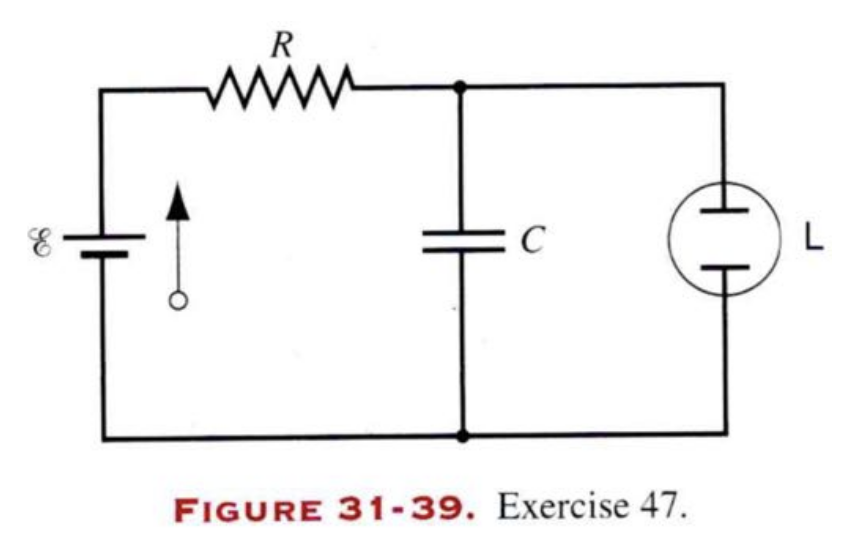
\includegraphics[scale=0.6]{31-39.png}
\end{center}
\end{problem}

\begin{solution}
\vfill
\end{solution}
\newpage

\end{document}
